\ylDisplay{Torud} % Ülesande nimi
{Jaan Kalda} % Autor
{piirkonnavoor} % Voor
{2010} % Aasta
{G 10} % Ülesande nr.
{9} % Raskustase
{
% Teema: Staatika
\ifStatement
Põrandale asetatakse kõrvuti kaks ühesugust silindrilist toru --- paralleelselt ja küljetsi üksteist puutuvana. Kolmas samasugune toru asetatakse nende peale --- samuti paralleelselt, nõnda et see toetub kahele alumisele.
Milliseid tingimusi peavad rahuldama hõõrdetegur $\mu$ toru ja põranda vahel ning hõõrdetegur $k$ kahe toru vahel
selleks, et pealmine toru kahte alumist üksteisest eemale ei vajutaks?

\begin{center}
	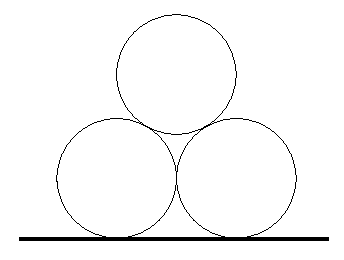
\includegraphics[width=0.3\linewidth]{2010-v2g-10-torud.eps}
\end{center}
\fi


\ifHint
Tasakaalu korral peab iga toru jaoks kehtima jõudude ning jõumomentide tasakaal. Alumiste torude jaoks on jõumomentide tasakaalu kõige mugavam vaadelda maapinna puutepunkti suhtes, sest sellisel juhul on maapinna hõõrdejõu panus \num{0}. Lisaks paneme tähele, et kahe alumise silindri vahel rõhumisjõudu ei ole, sest see kaob niipea, kui alumised silindrid natukenegi üksteisest eemalduvad.
\fi


\ifSolution
Kõigepalt paneme tähele, et põhimõtteliselt võiks antud süsteemis toimida rõhumisjõud kahe alumise silindri vahel, kuid see
kaob niipea, kui alumised silindrid natukenegi üksteisest eemalduvad; niisiis võime sellega mitte arvestada.

\begin{center}
	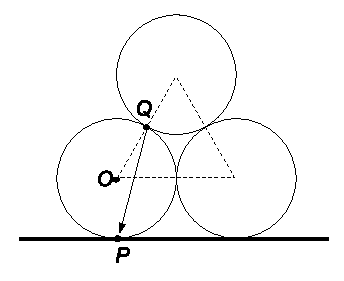
\includegraphics[width=0.6\textwidth]{2010-v2g-10-torudlah.eps}
\end{center}

Esmalt oletame, et $\mu$ on piisavalt suur, nii et vastu põrandat toetuvad torud pigem veerevad kui libisevad (kui $k$ pole piisavalt suur). Vaatleme vastu põrandat toetuvale torule mõjuvate jõumomentide tasakaalu tingimust toru ja põranda kontaktpunkti $P$ suhtes. Põranda rõhumis- ja hõõrdeju õlg on null; ka raskusjõud $mg$ õlg on null. Vaadeldavale torule mõjub veel vaid üksainus jõud --- ülemise toru põhjustatud hõõrde- ja rõhumisjõu resultant, mis on rakendatud puutepunkti $Q$ (vt joonist) ja kui tegemist on libisemise piirjuhuga (st veidigi väiksem hõõrdetegur $k$ viiks libisemisele), siis moodustab see vektor pinnanormaaliga nurga $\arctan k$ (sest antud vektor moodustub üksteisega risti olevate rõhumisjõu $N$ ja hõõrdejõu $F_h$ vektorite resultandina ning nurga tangens on $F_h/N=k$). Et ülejäänud jõudude moment oli null, siis peab ka selle jõu moment olema null,
st jõu vektor peab olema suunatud punkti $P$. Et kolmnurk $OQP$ on võrdhaarne (vt joonist),
siis
\[
k\ge \tan 15^\circ\approx \num{0,27}.
\]
Nüüd oletame, et $k \ge \tan 15^\circ$ ning vaatleme libisemise piirjuhtu punktis $P$. Selleks vaatleme jõumomentide tasakaalu punkti $Q$ suhtes.
Silindrile mõjuv raskusjõud $mg$ ning punktis $P$ toimiv rõhumisjõud $\frac 32 mg$ (mis kompenseerib poolteise silindri raskusjõu) on rakendatud sirge $OP$ sihis ning nende summaarne jõumoment $\frac 14mgR$ (kus $R$ on silindri raadius) tasakaalustab hõõrdejõu momendi 
\[
\frac 32 mg\mu \left(R+R\sin 60^\circ\right).
\]
Siinjuures arvestasime, et punktis $P$ toimiv hõõrdejõud on $\mu$-kordne rõhumisjõud $\frac 32 mg$ ning on horisontaalne ja omab seetõttu õlga $R+R\sin 60^\circ$. Seega,
\[
\mu \ge \frac{1}{6\left(1+\sin 60^\circ\right)}=\frac{1}{6\left(1+\frac{\sqrt 3}{2}\right)}\approx \num{0,09}.
\]
\fi
}